\documentclass[letterpaper]{article}



%%%%%%%%%%%%%%%%%%%%%%%%%%%%%%%%%%%%%%%%%%%%%%%%%
%%%%                  HI!                    %%%%
%%%%        THIS IS THE SSI-BIOLOGY			 %%%%
%%%%      GENERIC PROCEDURE TEMPLATE :) 	 %%%%
%%%%      IT MIGHT LOOK SCARY, BUT IT'S 	 %%%%
%%%%           PRETTY EASY TO USE 			 %%%%
%%%%%%%%%%%%%%%%%%%%%%%%%%%%%%%%%%%%%%%%%%%%%%%%%

%%%%%%%%%%%%%%%%%%%%%%%%%%%%%%%%%%%%%%%%%%%%%%%%%%%%%%%%%%
%%%%      RIGHT NOW YOU'RE LOOKING AT BOILERPLATE     %%%%
%%%%  THAT IS, THINGS YOU DON'T HAVE TO CHANGE (EVER) %%%%
%%%%     SCROLL DOWN FOR THE THINGS YOU SHOULD PAY    %%%%
%%%%    ATTENTION TO :)  (YOU'LL KNOW WHEN TO STOP)   %%%%
%%%%%%%%%%%%%%%%%%%%%%%%%%%%%%%%%%%%%%%%%%%%%%%%%%%%%%%%%%


%% Language and font encodings
\usepackage[english]{babel}
\usepackage[utf8x]{inputenc}
\usepackage[T1]{fontenc}

%% Sets page size, footer, indent and margins
\usepackage[a4paper,top=2.5cm,bottom=2cm,left=2.25cm,right=2.25cm,marginparwidth=2.25cm]{geometry}
\setlength\parindent{0pt}
\setlength{\footskip}{55pt}

%% Useful packages
\usepackage{amsmath}
\usepackage{graphicx}
\usepackage{fancyhdr}
\pagestyle{fancy}
\usepackage{textcomp}
\usepackage{gensymb}
%\usepackage{hyperref}
\usepackage{readarray}
\usepackage{verbatimbox}
\usepackage{framed}
\usepackage[dvipsnames]{xcolor}
\usepackage{tcolorbox}
\usepackage{colortbl}
\usepackage{libertine} 
\usepackage{siunitx}


% Safety Environment 
\definecolor{safetyFrame}{HTML}{FFFFFF}
\newenvironment{safety}{%
\begin{tcolorbox}[width=\textwidth, colframe=safetyFrame, arc=1.5mm]
}%
{\end{tcolorbox}}


% Footer
\lfoot{
\includegraphics[height=1.5cm]{1000x350-Horiz-Logo-WhiteRed-BlackText.png}}

% Substitution Commands
\newcommand{\tdt}{Terminal Deoxynucleotidyl Transferase}
\newcommand{\C}{\degree{}C}
\newcommand{\uL}{\micro{}L}
\newcommand{\BdATP}{3'-O-(2-nitrobenzyl)-2'-dATP}

%Custom Commands
\newcommand{\B}[1]{\textbf{#1}}

% Safety Info
\newcommand{\SYBRGold}{\item{\B{SYBR Gold} has no data available addressing the mutagenicity or toxicity of SYBR® Gold nucleic acid gel stain. Because this reagent binds to nucleic acids, it should be treated as a potential mutagen and handled with appropriate care. The DMSO stock solution should be handled with particular caution as DMSO is known to facilitate the entry of organic molecules into tissues.\cite{sybrGold}}}
\newcommand{\SYBRGreen}{\item{\B{SYBR Green I Gel Stain} binds to nucleic acids and is classified by the European Union as a mutagen of category 3. It should be handled with gloves and stored away from light at all times. The stock solution should be handled with particular caution as DMSO solvent is known to facilitate the entry of organic molecules into tissues.\cite{sybrGreenI}}}
\newcommand{\ETBR}{\item{\B{Ethidium Bromide} is a \B{serious mutagen} and is \B{significantly carcinogenic}. If working with considerable amounts, a \B{fume hood and respirator} are warranted. For more information see \url{https://www.sciencelab.com/msds.php?msdsId=9927667}
}}


% Shortcuts

%Stop Point (Optional)
\newcommand{\stopPoint}{\begin{center}
\rule{0.5\textwidth}{.4pt}\\
\vspace{1mm} 
OPTIONAL STOP POINT\\
\rule{0.5\textwidth}{.4pt}
\end{center}}

\newcommand{\RstopPoint}{\begin{center}
\rule{0.5\textwidth}{.4pt}\\
\vspace{1mm} 
RECOMMENEDED STOP POINT\\
\rule{0.5\textwidth}{.4pt}
\end{center}}

% Dilution Macro
\newcommand{\Dilution}[4]{
\subsection{#2}
\begin{enumerate}
\item{Vortex #2 stock}
\item{Pipette #1\uL{} #2 into a PCR Tube}
\item{Pipette #3\uL{} #4 into solution}
\item{Vortex until mixed}
%\item{Pipette $#2\mu L$ Water into solution}
\end{enumerate}
}

% Gel Macro
\newcommand{\gel}[4]{
\begin{figure}[ht]
\label{#3}
\begin{center}
\includegraphics[width=0.45\textwidth]{#1}
\includegraphics[width=0.45\textwidth]{#2}
\caption{#3}
\end{center}
\subsection{#3 Analysis}
#4
\end{figure}
}

% Well plate Macro
\newcommand{\wellplate}[2]{
\getargsC{#1}
\begin{tabular}{*{1}{>{\columncolor{blue!20}}l}|l|l|l|l|l|l|l|l|l|l|l|l|}
\rowcolor{blue!20}%
 & 1  & 2  & 3  & 4  & 5  & 6 & 7 & 8 & 9 & 10 & 11 & 12\\ \hline
\ifdefined\argxii
A & \argi & \argii & \argiii & \argiv & \argv & \argvi & \argvii & \argviii & \argix & \argx & \argxi & \argxii \\ \hline\fi
\ifdefined\argxxiv
B & \argxiii & \argxiv & \argxv & \argxvi & \argxvii & \argxviii & \argxix & \argxx & \argxxi & \argxxii & \argxxiii & \argxxiv \\ \hline\fi
\ifdefined\argxxxvi
C & \argxxv & \argxxvi & \argxxvii & \argxxviii & \argxxix & \argxxx & \argxxxi & \argxxxii & \argxxxiii & \argxxxiv & \argxxxv & \argxxxvi \\ \hline\fi
\ifdefined\argxlviii
D & \argxxxvii & \argxxxviii & \argxxxix & \argxl & \argxli & \argxlii & \argxliii & \argxliv & \argxlv & \argxlvi & \argxlvii & \argxlviii \\ \hline\fi
\ifdefined\arglx
E & \argxlix & \argl & \argli & \arglii & \argliii & \argliv & \arglv & \arglvi & \arglvii & \arglviii & \arglix & \arglx \\ \hline\fi
\ifdefined\arglxxii
F & \arglxi & \arglxii & \arglxiii & \arglxiv & \arglxv & \arglxvi & \arglxvii & \arglxviii & \arglxix & \arglxx & \arglxxi & \arglxxii \\ \hline\fi
\ifdefined\arglxxxiv
G & \arglxxiii & \arglxxiv & \arglxxv & \arglxxvi & \arglxxvii & \arglxxviii & \arglxxix & \arglxxx & \arglxxxi & \arglxxxii & \arglxxxiii & \arglxxxiv \\ \hline\fi
\ifdefined\argxcvi
H & \arglxxxv & \arglxxxvi & \arglxxxvii & \arglxxxviii & \arglxxxix & \argxc & \argxci & \argxcii & \argxciii & \argxciv & \argxcv & \argxcvi \\ \hline\fi
\end{tabular}
}

\usepackage[colorlinks]{hyperref}
\usepackage[colorinlistoftodos]{todonotes}
\usepackage{verbatim}

%%%%%%%%%%%%%%%%%%%%%%%%%%%%%%%%%%%%%%%%%%%%%%%
%%%%%%%%%%%%%%%%%%%%%%%%%%%%%%%%%%%%%%%%%%%%%%%
%%%%%%%%%%%%% End of Boiler Plate %%%%%%%%%%%%%
%%%%%%%%%%%%%%%%%%%%%%%%%%%%%%%%%%%%%%%%%%%%%%%
%%%%%%%%%%%%%%%%%%%%%%%%%%%%%%%%%%%%%%%%%%%%%%%

%%%%%%%%%%%%%%%%%%%%%%%%%%%%%%%%%%%%%%%%%%%%%%%
%%%%%   AKA YOU WRITE AFTER THIS POINT    %%%%%
%%%%%%%%%%%%%%%%%%%%%%%%%%%%%%%%%%%%%%%%%%%%%%%


\title{SSI Biology PCR Workshop} % CHANGE THIS
\author{Written by \textbf{Cynthia Hao and Alan Tomusiak}\\ % CHANGE THIS 
\\ % CHANGE THIS
        For the Stanford Student Space Initiative Biology Subteam}

\begin{document}

\maketitle

\section{Procedure Purpose} % CHANGE THIS
Basic polymerase chain reaction (PCR) and agarose gel electrophoresis workshop procedure.

\section{Overview} % CHANGE THIS
Amplify the ampicillin resistance gene (about 1000bp) from a plasmid using Polymerase Chain Reaction, and image the results on a 1\% agarose gel.

% Safety First! ALSO, % CHANGE THIS
\section{Safety Information}
\begin{safety}
\begin{enumerate}
%\SYBRGreen{} 
\item{Working in a communal lab space is hazardous. Do not assume your fellow workers cleaned up sufficiently, and be sure to sign into and out of lab with a lifeguard or SSI safety officer.}
\end{enumerate}
\end{safety}

\section{Materials}
\begin{enumerate}
\item{precast 1\% agarose gels}
\item{6x Purple Loading Dye}
\item{.5x TBE Buffer}
\item{1 uM forward primer}
\item{1 uM reverse primer}
\item{.1 ng/\uL{} pBR322 plasmid template DNA}
\item{.25 U/\uL{} Taq polymerase}
\item{5 mM dNTP Mix}
\item{10x Taq PCR buffer}
\item{nuclease-free water}
\item{1kb prestained DNA ladder working stock}
%\item{10x SYBR Green I}
\item{Bio-Rad gel apparatus and power supply}
\item{Thermal Cycler}
\item{Gel Imager}
\end{enumerate}

%\section{Dilutions} % We have a dilution macro! (courtesy of me, aka if you have a suggestion tell me please)
%\Dilution{2.5}{Primer 1}{22.5}{Water} % \Dilution{amount of liquid 1}{liquid1}{amount of liquid 2}{liquid2}

% Now for the _good_ stuff  
\section{Pipetting}
We're about to get started, but first, a quick note about pipetting:

\begin{center}
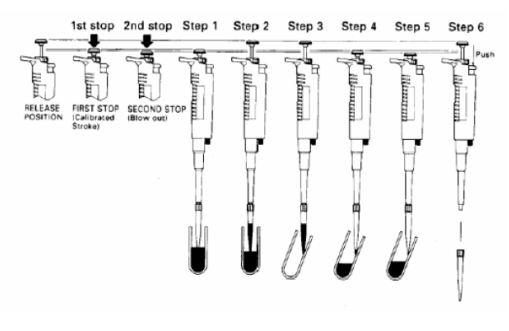
\includegraphics[width=.6\textwidth]{Capture.JPG}
\end{center}
\section{PCR Procedure}% CHANGE THIS
\begin{enumerate} % THIS STARTS THE "STEP SECTION"
\item{Obtain aliquots of Taq buffer, dNTP mix, forward primer, reverse primer, template DNA, and Taq polymerase for your group from the reagent ice bucket.}
\item{Label two PCR tubes with your initials.}
\item{For each person: Pipette 15 \uL{} water, 5 \uL{} 10x Taq buffer, 2 \uL{} 5 mM dNTP mix, 10 \uL{} each 1 uM reverse primer stock and forward primer stock, 3 \uL{} (.3 ng) of plasmid template DNA, and 5 \uL{} Taq polymerase stock into each PCR tube, in that order. The total reaction volume should be 50 \uL{}.}
%\item{5 \uL{} 10x SYBR Green replaces 5 \uL{} water for real time PCR}
\begin{table}[ht]
\centering
\caption{PCR reaction concentrations}
\label{my-label}
\begin{tabular}{|l|l|l|l|}
\hline
Reagent        & Stock Concentration & Desired Concentration & Volume (\uL{}) \\ \hline
Water          &                     &                       & 15       \\ \hline
Taq Buffer     & 10x                 & 1x                    & 5           \\ \hline
dNTP Mix       & 5 mM               & 200 uM                & 2           \\ \hline
Forward Primer & 1 uM               & .2 uM                 & 10         \\ \hline
Reverse Primer & 1 uM               & .2 uM                 & 10         \\ \hline
Template DNA   & .1 ng/\uL{}             & .3 ng/50 \uL{} reaction   & 3           \\ \hline
%SYBR Green I   & 10x                 & 1x                    & 5           \\ \hline
Taq Polymerase & .25 U/\uL{}            & 1.25 U/50 \uL{} reaction & 5         \\ \hline
Total          &                     &                       & 50          \\ \hline
\end{tabular}
\end{table}

\item{Pipette up and down thoroughly in each tube to mix. Do not press down to the second pipette stop.}
\item{Place your PCR tubes in the thermal cycler, starting from the top left position and filling in column by column.}
\item{Get an SSI member to help you program in the following temperature protocol for a gradient PCR:}
%\item{Transfer each reaction from the PCR tube into one well of a 96-well plate. Fill in the plate column by column, starting from A1.}
%\item{Place the 96-well plate into the qPCR machine and get an SSI member to help you program in the following temperature protocol:}

\begin{table}[h!]
\centering
\caption{Gradient PCR Temperature Protocol}
\label{my-label}
\begin{tabular}{|l|l|l|}
\hline
Step                       & Temperature (C) & Time     \\ \hline
Initial Denaturation       & 98          & 30 sec   \\ \hline
Denaturation               & 98          & 30 sec   \\ \hline
Annealing (depends on primer melting temperature)                 & 46-60       & 30 sec   \\ \hline
Extension (1 min per 1kb product)                 & 72          & 1 min    \\ \hline
GOTO Denaturation Step 29 times &             &          \\ \hline
Final Extension            & 72          & 10 min   \\ \hline
Hold                       & 4           & Infinity \\ \hline
\end{tabular}
\end{table}

\item{This protocol will set up a temperature gradient from 46-60C, with a different temperature for each row of the thermal cycler for the annealing step.}
%\item{Observe SYBR Green signal using the qPCR machine to determine the results of your PCR. You should see a logarithmic fluorescence curve if your PCR was successful.} 
\end{enumerate}

\section{Gel Electrophoresis Procedure}
\begin{enumerate}
\item{Obtain a pre-cast, SYBR Green pre-stained 1\% agarose gel, 1kb ladder working stock for the group, and 1 PCR tube of DNA sample for gel electrophoresis per group.} 
\item{Position the gel in the gel apparatus so that the wells are closer to the negative electrode, and fill the gel apparatus with .5x TBE buffer so that it completely covers the gel.}
\item{Obtain a piece of parafilm for your group. Draw a labeled grid on the parafilm with 9 boxes (3 for each person in the 3-person group). Keep track of where you are pipetting.} 
\item{Each person in the group should pipette one 2 \uL{} droplet of 6x Purple Loading Dye onto the parafilm into each of three boxes.}
\item{Pipette 5 \uL{} of 0.5x TBE buffer into each of three loading dye droplets.}
\item{Pipette 5 \uL{} of the appropriate sample into each of three loading dye droplets.}
\item{As you go, pipette up and down to mix thoroughly. Be sure not to press down to the second stop.}
\item{Load 5\uL{} of the prestained ladder mix directly from the aliquot into the first well of the gel. Ensure pipette tip is in the well but does not puncture the bottom, and depress slowly and carefully to avoid bubbles.}
\item{Each person should load 5\uL{} of their three PCR sample droplets into the next three wells of the gel.}

\begin{figure}[ht]
\begin{center} 
\addvbuffer[{0mm} \baselineskip]{\begin{tabular}{|l|l|}
\hline
Well number    & Sample \\ \hline
1                                  & 1 kb Ladder (control)   \\ \hline
2                                  & Person 1 DNA Sample 1   \\ \hline
3                                  & Person 1 DNA Sample 2  \\ \hline
4                                  & Person 1 DNA Sample 3  \\ \hline
5                                  & Person 2 DNA Sample 1    \\ \hline
6                                  & Person 2 DNA Sample 2    \\ \hline
7                                  & Person 2 DNA Sample 3  \\ \hline
8                                  & Person 3 DNA Sample 1  \\ \hline
9                                  & Person 3 DNA Sample 2  \\ \hline
10                                  & Person 3 DNA Sample 3  \\ \hline
\end{tabular}}
\label{tab:Gel Layout}
\caption{Gel Layout} 
\end{center}
\end{figure}
\item{Cover the gel with the lid and plug the gel into the power supply.}
\item{Run the gel at 120V until the red portion (the first front) of the loading dye is at least 50\% of the way to the other side of the gel.}
\item{Proceed to imaging. Have an SSI member help you position the gel in the gel imager, ensure correct gel orientation with the wells on the left side, and enter in the imaging protocol, optimizing for intense bands with SYBR Green pre-stain.}
\item{Note down how many bands you see, the length of the bands, and whether or not the PCR was successful.}
\item{Wipe down the gel imager with kimwipes and ethanol.}
\item{Clean up your lab station, replace reagents in freezer or room temperature storage, throw pipette tips in regular trash, put pipette boxes back in the drawers, rinse out gel boxes, and refill buffer stock with .5x TBE buffer.}
\item{Sign out of lab with the appropriate google form.}
\end{enumerate}
%\bibliographystyle{ieeetr}
%\bibliography{biblio}
\end{document}